\documentclass{standalone}
%\pagenumbering{gobble}


%%%%%%%%%%%%%%%%%%%%%%%%%%%%%%%%%%%%%%%%%%%%
%
% schematic of pressure driven shock
% in dynamically expanding HII region
%
%
%%%%%%%%%%%%%%%%%%%%%%%%%%%%%%%%%%%%%%%%%%%%


\usepackage{tikz}
\usepackage[outline]{contour}
\usetikzlibrary{arrows, snakes, calc}
\usetikzlibrary{shapes.geometric}

%[draw options] (center) (initial angle:final angle:radius)
\def\centerarc[#1](#2)(#3:#4:#5) {\draw[#1] ($(#2)+({#5*cos(#3)},{#5*sin(#3)})$) arc (#3:#4:#5);}

%[draw options] (center) (initial angle:final angle:inner radius:outer radius)
\def\myarc[#1](#2)(#3:#4:#5:#6) {\draw[#1] ($(#2) + (#3:#5)$) arc (#3:#4:#5)
		--  ($(#2) + (#4:#6)$) arc (#4:#3:#6) -- cycle;}

\begin{document}

\tikzset{
	trans/.style={very thick, dashed,->,shorten >=2pt,shorten <=0pt,>=stealth},
	photon/.style={very thick, ->, snake=snake, line after snake=1mm}
	}


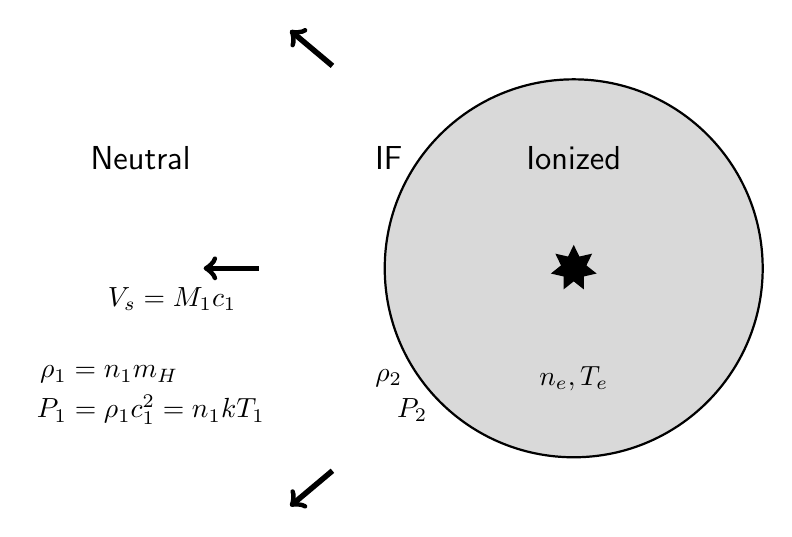
\begin{tikzpicture}[scale=1.0, font=\sffamily]

	\draw[thick, fill=gray!30] (0,0) circle (2.4);
	%\myarc[white, fill=white](0,0)(125:235:2.4:3.1)
	\centerarc[line width=0.7mm, dashed](0,0)(125:235:3.1)
	\myarc[gray!20, fill=gray!20](0,0)(125:235:3.1:3.5)
	\myarc[gray!50, fill=gray!50](0,0)(125:235:3.5:3.8)
	\myarc[gray!90, fill=gray!90](0,0)(125:235:3.8:4.0)
	\myarc[fill=black](0,0)(125:235:4.0:4.1)
	\node[star,star points=7,star point ratio=1.8, fill] at (0,0) {};

	\node at (0,1.4) {\large{Ionized}};
	\node at (0,-1.4) {$n_e, T_e$};
	%\node at (0,-1.4) {$n_e < n_1$};
	%\node at (0,-1.8) {$T_e$};
	\node at (-5.5,1.4) {\large{Neutral}};
	\node at (-5.9,-1.35) {$\rho_1 = n_1 m_H$};
	\node at (-5.37,-1.8) {$P_1 = \rho_1 c_1^2 = n_1kT_1$};
	\node at (-2.35,1.4) {\large{IF}};
	\node at (-2.35,-1.4) {$\rho_2$};
	\node at (-2.05,-1.8) {$P_2$};

	%\draw[rotate=115, dashed, <->] (0,0) -- ++(0,2.4);
	%\node[rotate=0] at (-1.2,-0.8) {$R$};
	%\draw[rotate=115, dashed, <->] (0,2.4) -- ++(0,0.7);
	%\node[rotate=0] at (-2.4,-1.35) {$\Delta R$};
	\node[rotate=0, align=right] at (-5.1,-0.39) {$V_s = M_1 c_1$};

	%\draw[photon, rotate=65] (0,0) -- ++(0,1.1);
	%\node[rotate=0, align=right] at (-0.25,0.65) {$\dot N_{ionize}$};
	%\draw[photon, rotate=65] (0,2.0) -- ++(0,0.8);
	%\node[rotate=0] at (-2.3,1.45) {$\dot N$};

	\draw[line width = 0.7mm, rotate=90, ->] (0,4.0) -- ++(0,0.7);
	\draw[line width = 0.7mm, rotate=130, ->] (0,4.0) -- ++(0,0.7);
	\draw[line width = 0.7mm, rotate=50, ->] (0,4.0) -- ++(0,0.7);

\end{tikzpicture}
\end{document} 
